\paragraph{QuizziPedia::Back-End::App::Controllers::NotFoundHandler}
\label{QuizziPedia::Back-End::App::Controllers::NotFoundHandler}
\begin{figure}[ht]
	\centering
	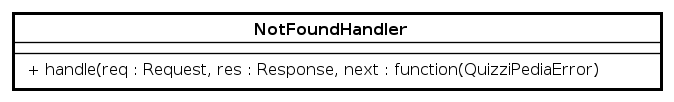
\includegraphics[scale=0.45]{UML/Package/QuizziPedia_Back-End_App_Controllers_notFoundHandler.png}
	\caption{QuizziPedia::Back-End::App::Controllers::NotFoundHandler}
\end{figure}
\FloatBarrier
\begin{itemize}
	\item \textbf{Descrizione}:
	classe che si occupa della gestione dell'errore di pagina non trovata. Componente \textit{ConcreteHandler\ped{G}} del \textit{design pattern\ped{G}} \textit{Chain of responsibility\ped{G}}.
	\item \textbf{Utilizzo}:
	viene utilizzata per generare una pagina 404 di errore nel caso in cui l'\textit{URI\ped{G}} passato non corrisponda ad una risorsa presente nell'applicazione.
	\item \textbf{Relazione con altre classi}:
	\begin{itemize}
		\item \textbf{IN} \texttt{UserRouter}:
		classe che gestisce le richieste relative alle operazioni riguardanti l'utente. Componente \textit{ConcreteHandler\ped{G}} del \textit{design pattern\ped{G}} \textit{Chain of responsibility\ped{G}};
		\item \textbf{IN} \texttt{QuestionRouter}:
		classe che gestisce le richieste relative alle operazioni riguardanti le domande. Componente \textit{ConcreteHandler\ped{G}} del \textit{design pattern\ped{G}} \textit{Chain of responsibility\ped{G}};
		\item \textbf{IN} \texttt{QuizRouter}:
		classe che gestisce le richieste relative alle operazioni riguardanti i questionari. Componente \textit{ConcreteHandler\ped{G}} del \textit{design pattern\ped{G}} \textit{Chain of responsibility\ped{G}}.
	\end{itemize}
	\item \textbf{Metodi}:
	\begin{itemize}
		\item \texttt{+ handle(req: Request, res: Response, next: function(QuizziPediaError))}\\
		Metodo che gestisce la costruzione dei messaggi d'errore ritornando un JSON contenente il messaggio d'errore.\\
		\textbf{Parametri}:
		\begin{itemize}
			\item \texttt{req: Request}\\
			Rappresenta la richiesta inviata al \textit{server\ped{G}};
			\item \texttt{res: Response}\\
			Rappresenta la risposta che il \textit{server\ped{G}} fornirà al termine dell'esecuzione del metodo;
			\item \texttt{next: function(QuizziPediaError)}\\
			Rappresenta la \textit{callback\ped{G}} che il metodo deve chiamare al termine dell'elaborazione per passare il controllo ai successivi middleware. La presenza del parametro facoltativo \texttt{QuizziPediaError} attiva la catena di gestione dell'errore in sostituzione della normale catena di gestione delle richieste.
		\end{itemize}
	\end{itemize}
\end{itemize}

